%%% Local Variables:
%%% mode: latex
%%% TeX-master: "../main"
%%% End:

\section{Methodology}
This section outlines the implementation details of the voxel rendering engine, starting from the selection of programming languages and libraries, going over the architecture of the engine, and diving deep into the data structures and algorithms employed, particularly focusing on VDB for voxel representation and the optimization of ray casting algorithms.
Finally, this section will discuss the extension of these algorithms to full-fledged ray tracing, allowing for dynamic lightning and glossy material support.

\subsection{Rust \& wgpu}
\hyphenation{WebGPU}

The voxel rendering engine is built using \textbf{Rust}, a programming language known for its focus on safety, speed, and concurrency\supercite{rustbook}.
Rust's design emphasizes memory safety without sacrificing performance, making it an excellent choice for high-performance applications like a rendering engine.
The language's powerful type system and ownership model prevent a wide class of bugs, making it ideal for managing the complex data structures and concurrency challenges inherent in rendering engines. Thanks to this no memory leak or null pointer was ever encoutered throughout the developmenent of this project.

For the graphical backend, the engine utilizes \textbf{wgpu}\supercite{wgpu:doc}, a Rust library that serves as a safe and portable graphics API. wgpu is designed to run on top of various backends, including Vulkan, Metal, DirectX 12, and WebGL, ensuring cross-platform compatibility. This API provides a modern, low-level interface for GPU programming, allowing for fine-grained control over graphics and compute operations. wgpu is aligned with the WebGPU specification\supercite{webgpu:doc}, aiming for broad support across both native and web platforms.
This choice ensures that the engine can leverage the latest advancements in graphics technology while maintaining portability and performance.

The combination of Rust and wgpu offers several advantages for the development of a rendering engine:

\begin{enumerate}
  \item \emph{Safety and Performance:} Rust’s focus on safety, coupled with wgpu's design, minimizes the risk of memory leaks and undefined behaviors, common issues in high-performance graphics programming. This is thanks to Rust's idea of zero-cost abstractions.

  \item \emph{Cross-Platform Compatibility:} With wgpu, the engine is not tied to a specific platform or graphics API, enhancing its usability across different operating systems and devices.

  \item \emph{Future-Proofing:} wgpu's adherence to the WebGPU specification ensures that the engine is built on a forward-looking graphics API, designed to be efficient, powerful, and broadly supported. It also allows the future option of supporting web platforms, once browsers adopt WebGPU more throughly.

  \item \emph{Concurrency:} Rust’s advanced concurrency features enable the engine to efficiently utilize multi-core processors, crucial for the heavy computational demands of rendering pipelines.
\end{enumerate}

These technical choices form the foundation upon which the voxel rendering engine is constructed. Following this, the engine's architecture is designed to take full advantage of Rust's performance and safety features and wgpu's flexible, low-level graphics capabilities, setting the stage for the implementation of advanced voxel representation techniques and optimized ray tracing algorithms.


\subsection{Engine architecture}

The engine's operation is centered around an event-driven main loop that blocks the main thread.
This loop processes various events, ranging from keyboard inputs to redraw requests, and updates the window, context, and scene accordingly, routing each event to it's corresponding handler.

\begin{figure}[H]
  \centering
  \includesvg[width=0.5\linewidth]{engine_1}
  \caption{Engine event-loop diagram. Dotted arrows are implemented in \texttt{winit} crate. Black lines represent the flow of events. The arrow line represents the main render function called on the GPU context on the scene for the window.}
\end{figure}


\subsubsection{Runtime}
\newacronym{os}{OS}{Operating System}
\begin{samepage}
At the engine's core, sits \texttt{Runtime}  structure, which manages the interaction between the it's main components:
\begin{itemize}
  \item The \texttt{Window} is a handler to the engine's graphical window. It is used in filtering \acrshort{os} events that relevant to engine, grabbing the cursor and other boilerplate.
  \item The \texttt{Wgpu Context} holds the creation and application of the rendering pipeline.
  \item The \texttt{Scene} contains information abput the camera and enviorment as well as a container voxel data structure.
\end{itemize}
\end{samepage}

\begin{lstlisting}[language=rust,caption={Runtime definition},captionpos=b]
pub struct Runtime {
  context: WgpuContext,
  window: Window,
  scene: Scene,
}

impl Runtime {
  ...
  pub fn main_loop(&mut self, event: Event, ...) {
    match event {
      ...
    }
  };
}
\end{lstlisting}


For example, window events (e.g. keyboard \& mouse input) generaly modify the scene, like the camera position, and therfore are routed to the \verb|Scene| struct.

Another key event is the \verb|RedrawRequested| event, which signals that a new frame should be rendered. This is routed to the wgpu context to start the rendering pipeline.

The \verb|RedrawRequested| event is actually emmited in \verb|Runtime|, when it receives the \verb|MainEventsCleared| event, it scheduels the window for a redraw.

\subsubsection{Window}
The \verb|Window| data structure, included in the \textbf{winit}\supercite{winit:doc} crate, handles window creation and management, and provides an interface to the GUI window through an event loop. This event loop is what \verb|Runtime|'s main loop is mounted on.

The interaction between the \verb|Window| and the \verb|Runtime| forms an event-driven workflow. The window emmits events and the runtime manages and distributes these events accordingly, forming a sort of feedback loop.

\subsubsection{Scene}
The \verb|Scene| data structe holds information about the enviorment that is being rendered, this includes the model, camera, and engine state.

\begin{lstlisting}[language=rust,caption={Scene definition},captionpos=b]
pub struct Scene {
    pub state: State,
    pub camera: Camera,
    pub model: VDB,
}
\end{lstlisting}

In this section, the camera and satte implementation is covered, the model will be covered in later [add link] when discussing the \acrshort{vdb} implementation.
\newacronym{fps}{FPS}{Frames per second}
\newacronym{fov}{FOV}{Field of view}

\paragraph{State} handles information about the engine state such as cursor state and time synchronising to decouple engine events from the \acrshort{fps} (e.g. camera movement shouldn't be slower at lower FPS).

\paragraph{Camera} describes all the elements needed to control and represent a camera:
\begin{enumerate}
    \item \emph{Eye:} The camera's position in the 3D space, acting as the point from which the scene is observed.
    \item \emph{Target:} The point in space the camera is looking at, determining the direction the camera is pointed in.
    \item \emph{Field of View (FOV):} An angle representing the range that is in view. In the implementation, this refers to the FOV on the $Y$ (vertical) axis.
    \item \emph{Aspect ratio:} The ratio between the width and height of the viewport. It esnures that the rendered scene maintains the correct proportions.
\end{enumerate}
The eye and target are updated when moving the camera through a \verb|CameraController| struct that handles keyboard and mouse input. Th FOV and aspect ratio are set based on the window proportions, to avoid distortion. The way in which this camera information is used will be detailed in the primitives section [add link] where we dive into what information is actually sent to the GPU in compute shaders.


\subsubsection{WgpuContext}
The \verb|WgpuContext| structure is the backbone of the rendering pipeline in the voxel rendering engine. It contains the necessary components for interfacing with the GPU using the wgpu API, managing resources such as textures, shaders, and buffers, and executing rendering commands.

Broadly, \verb|WgpuContext| has the follwing responsablities:
\begin{enumerate}
  \item \emph{Initialization:} The constructor sets up the wgpu instance, device, queue, and surface.
        It also configures the surface with the desired format and dimensions, preparing the context for rendering.
  \item \emph{Resource Setup:} The constructor prepares various resources such as textures for the atlas representation of VDB data, uniform buffers for rendering state, and bind groups for shader inputs.
        It also dynamically reads VDB files, processes the data, and updates GPU resources accordingly.
  \item \emph{Rendering:} The render method handles updating the window surface.
        It triggers compute shaders for voxel data processing, manages texture and buffer updates, and executes the render pipeline. Additionally, it manages shader hot-reloading, renders the developer GUI and handles screen capture for recording.
\end{enumerate}

\subsubsection{Graphichs Pipeline}
This section provides an overview of the graphics pipline that is initiated at a \verb|RedrawRequest| event.

\begin{figure}[H]
\noindent\begin{minipage}[t]{0.65\textwidth}
  \vspace{0.5cm}
  When the \verb|WgpuContext|'s render method is invoked, it starts by obtaining a reference to the output texture and creates a corresponding view. Following this, a command encoder is initialized to record GPU commands.

  Next, it uses the \verb|FrameDescriptor|, a structure designed to transform scene information (including the model, camera, and engine state), stored on the CPU, into GPU-compatible bindings. This step prepares all necessary bindings for the compute shaders, which then execute the ray-tracing algorithm across distributed workgroups, with the results written to a texture.

  Once computation is complete, the texture containing the rendered image is prepared for display. This involves creating a vertex shader to generate a full-screen rectangle, onto which the texture is rasterized using fragment shaders, effectively transferring the rendered image to the output texture.

  The final phase involves adding the GUI layer over the rendered scene before presenting the completed output texture on the screen.

\end{minipage}
\hfill
\begin{minipage}[t]{0.3\textwidth}
  \vspace{-0.5cm}
  \begin{figure}[H]
    \centering
    \includesvg[width=\linewidth]{pipeline}
  \end{figure}
\end{minipage}
\end{figure}

\subsubsection{GPU Types}
This section covers the \verb|FrameDescriptor| data structe and how it generates GPU bindings from the data in \verb|Scene| which is stored on the CPU.

Virtually the entire ray-tracing algorithm is run in compute shaders. This means all the information about the model, camera, lights, and metadata has to be passed through.

The statically sized data i.e. the camera, sunlight and metadata is passed in an uniform buffer. This buffer is assembled inside the \verb|FrameDescriptor| which wraps \verb|ComputeState|.
This is a data structure that converts bla bla.
Matrix Conversion: The camera's view projection matrix and the transformation from camera to world coordinates are flattened into 4x4 f32 arrays.
Camera Position and Orientation: The camera's position (eye) and orientation vectors (u, -v, and w') are represented as arrays, facilitating the calculation of ray directions within the compute shader.
Rendering Parameters: Additional fields such as render\_mode, show\_345 (a flag array for toggling voxel boundary highlighting), sun\_dir, and sun\_color (with the alpha channel representing intensity) are included to control various aspects of the rendering process, from the mode of rendering to the simulation of lighting conditions.



\subsubsection{Camera}

\subsubsection{Shaders}
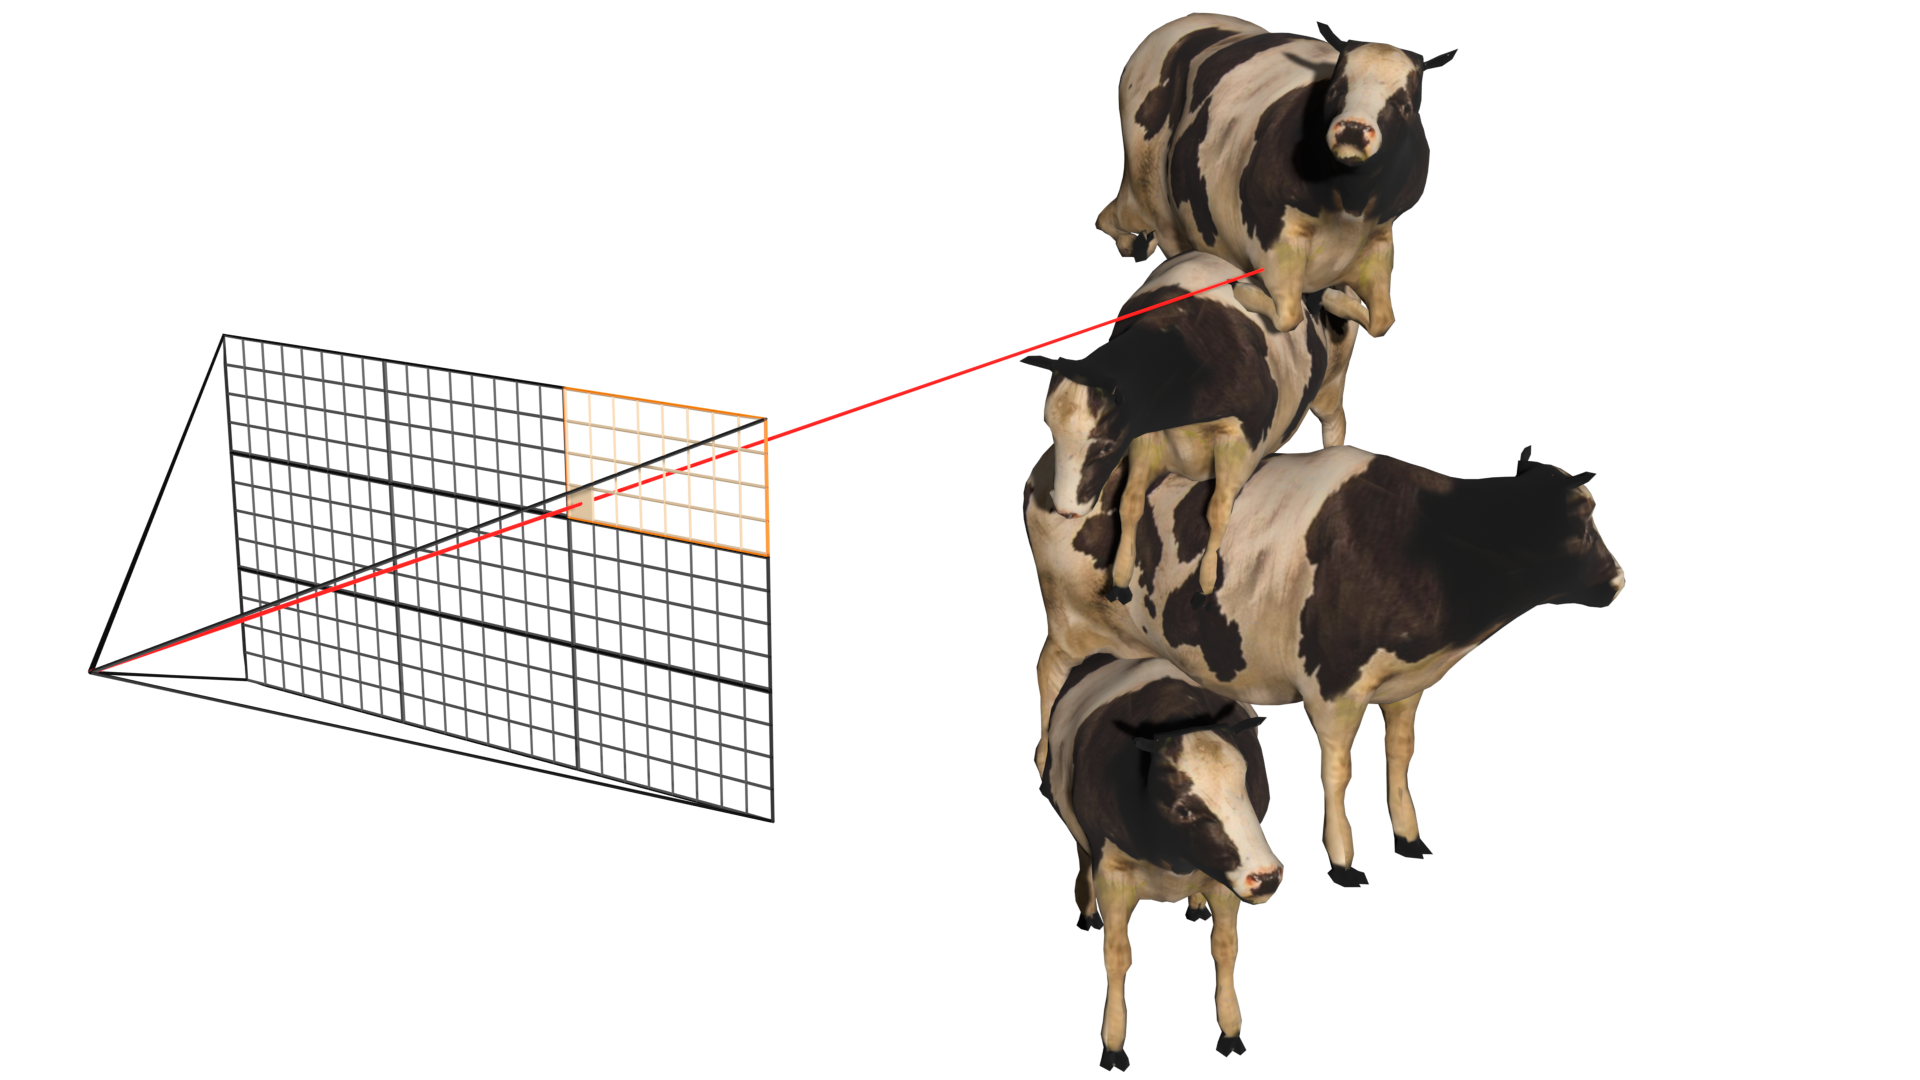
\includegraphics[width=1.0\linewidth]{compute_shaders}

\subsubsection{Utilities}

\subsection{VDB Implementation}
